% -----------------------------------------------------------------
% Vorlage fuer Ausarbeitungen von
% Bachelor- und Masterarbeiten am ISS
% 
% Template for written reports or master theses at the ISS
% 
% For use with compilers pdflatex or latex->dvi2ps->ps2pdf.
%
% -----------------------------------------------------------------
% README, STUDENT USERS:
% We highly appreciate students using this template _AS IS_,period. 
% The document provides adjustable document preferences, 
% student information settings and typography definitions. Look for
% code delimited by *** ***
%
% The short explanation: it's the ISS common standard and 
% 	it's battle tested.
% The long explanation: 
%	We do not want you to go through the document and tweak the 
%	package options, layout parameters and line skips here and 
%	there and waste hours. We are providing this template such 
%	that you can fully concentrate on filling in the much more 
%	important _contents_ of your thesis.
%
% If you have serious needs on extra packages or design 
% modifications, talk to your supervisor _before_ modifying 
% the template.
% Similarly, we're happy if you give your supervisor a hint on any 
% errors in this template.
%
% -----------------------------------------------------------------
% History:
% Jan Scheuing,   04.03.2002
% Markus Buehren, 20.12.2004
% last changes:   10.01.2008 (removed unused packages), 
% 		07.08.2009 (added IEEEtran_LSS.bst file)
% 		02.05.2011 removed matriculation number from cover page
% Martin Kreissig, 25.01.2012, all eps/ps parts removed for 
% 				pdflatex to work properly
% Peter Hermannstaedter, 14.08.2012, fusion of versions for 
% 		latex/dvi/ps/pdf and pdflatex, additional comments,
% 		unification of document flags and student options
%
% -----------------------------------------------------------------
% To do: 
% - remove obsolete documentclass options if all our systems 
%	have up-to-date tex distributions
% -----------------------------------------------------------------


\documentclass[12pt,DIV14,BCOR12mm,a4paper,footexclude,headinclude,halfparskip-,twoside,openright,openany,cleardoubleempty,idxtotoc,bibtotoc]{scrreprt} % Koma-Script
%
%
%
% *****************************************************************
% -------------------> document preferences here <-----------------
% *****************************************************************
% Uncomment the settings you like and comment the settings you dont
% like.

% Language: 
% affects generic titles, Figure term, titlepage and bibliography
% (Note:if you switch the language, compile tex and bib >2 times)
\def \doclang{english} 	% For theses/reports in English
%\def \doclang{german} 		% For theses/reports in German

% Hyperref links in the document:
\def \colortype{color} % links with colored text
%\def \colortype{bw} 	% plain links, standard text color (e.g. for print)
%\def \colortype{boxed} % links with colored boxes
% *****************************************************************
%
%
%
% *****************************************************************
% --------------> put student information here <------------------
% *****************************************************************
% Pleas fill in all items denoted by "to be defined (TBD)"
\def \deworktitle{Vergleich von aktuellen Clustering Algorithmen}        % German title/translation
\def \enworktitle{Comparison of State-of-the-art Clustering algorithm}       % English title/translation
\def \tutor{Alexander Bartler}
\def \student{Simon Kamm}
\def \worksubject{Research Thesis s1279}
\def \startdate{22.10.2018}
\def \submission{21.04.2019}
\def \signagedate{21.04.2019}   % Date of signature of declaration on last page
\def \keywords{deep learning, unsupervised learning, clustering, autoencoder, variational autoencoder, kmeans, gaussian mixture model}
\def \abstract{Current "state-of-the-art" clustering algorithms are usually consist of two parts. The first one is a dimensionality reduction (often called feature extraction) part while the second one uses the extracted features and perform clustering on those. In this work, selected "state-of-the-art" clustering models based on different autoencoder models are implemented. A large-scale evaluation for this models is done to check their performance on (more and less) complicated datasets (from 32x32 greyscale images of MNIST \cite{MNIST-Data} to 64x64 rgb images of IMAGENET \cite{imagenet_cvpr09}). Additionally the effect of different hyperparameter settings is investigated. Hyperparameters are separated into two kinds of hyperparameters. They are separated into model-related hyperparameters, which directly influence the model (i.e. size of latentspace) and training-related hyperparameters (i.e. learning rate schedule, batch size, etc.). Firstly, the specific model-related hyperparameters are optimized based on "basic" training-related hyperparameters. Secondly, the model-related hyperparameters will be fixed and the second set of hyperparameters will be varied and their impact on the clustering performance will be investigated.
In this work state-of-the-art algorithms will be investigated, implemented and optimized inside a self-programmed framework (in Tensorflow) with comparative model architectures and training procedure. These different models are then evaluated with different hyperparameters on different Datasets.}
% \def \studentID{Matriculation number}  % matriculation number on cover sheet deprecated (2011-05-02)

% *****************************************************************
%
%

\usepackage[latin1]{inputenc}
\usepackage{amsmath}
\usepackage{amsfonts}
\usepackage{ifthen}
\ifthenelse{\equal{\doclang}{german}}{
	\usepackage[ngerman]{babel} %german version!!
	\def \langtitle{\enworktitle}
	%\def \suptitle{\enworktitle}	
}{
	%english version!!
	\def \langtitle{\enworktitle}
	\def \suptitle{\deworktitle}
}
\usepackage{txfonts} % Times-Fonts
\usepackage[T1]{fontenc}
\usepackage{color}
\usepackage[headsepline]{scrpage2} % Headings

\usepackage{graphicx}
\usepackage[format=hang]{caption}       % for hanging captions
\usepackage{subfig}                     % for subfigures
\usepackage{wrapfig}                    % for figures floating in text, alternatively you can use >>floatflt<<
\usepackage{booktabs}
\usepackage{algorithm}
\usepackage{algorithmic}

\ifthenelse{\equal{\colortype}{color}}{
	% colored text version:
	\usepackage[colorlinks,linkcolor=blue]{hyperref}
	\newcommand{\bugfix}{\color{white}{\texttt{\symbol{'004}}}} % Bug-Fix Umlaute in Verbatim
}{
	\ifthenelse{\equal{\colortype}{boxed}}{
		% colored box version:
		\usepackage{hyperref}
		\newcommand{\bugfix}{\color{white}{\texttt{\symbol{'004}}}} % Bug-Fix Umlaute in Verbatim
	}{
		% monochrome version:
		\usepackage[hidelinks]{hyperref}
		\newcommand{\bugfix}{\color{white}{\texttt{\symbol{'004}}}} % Bug-Fix Umlaute in Verbatim
	}
}

% Layout and Headings
\pagestyle{scrheadings}
\automark{chapter}
\clearscrheadfoot
\lehead[]{\pagemark~~\headmark}
\rohead[]{\headmark~~\pagemark}
\renewcommand{\chaptermark}[1]{\markboth {\sl \hspace{8mm}#1}{}}
\renewcommand{\sectionmark}[1]{\markright{\sl \thesection~#1\hspace{8mm}}}
\addtolength{\textheight}{15mm}
\parindent0ex
\setlength{\parskip}{5pt plus 2pt minus 1pt}
\renewcommand*{\pnumfont}{\normalfont\slshape} % Seitenzahl geneigt
\renewcommand*{\sectfont}{\bfseries} % Kapitelueberschrift nicht Helvetica

% Settings for PDF document
\pdfstringdef \studentPDF {\student}
\pdfstringdef \worktitlePDF {\langtitle}
\pdfstringdef \worksubjectPDF {\worksubject}
\hypersetup{pdfauthor=\studentPDF, 
	pdftitle=\worktitlePDF,
	pdfsubject=\worksubjectPDF}

% Title page
\titlehead{
	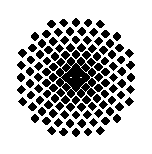
\includegraphics[width=20mm]{university-logo}
	\hspace{6mm}
	\ifthenelse{\equal{\doclang}{german}}{
		\begin{minipage}[b]{.6\textwidth}
			{\Large Universit\"at Stuttgart } \\
			Institut f\"ur Signalverarbeitung und Systemtheorie\\
			Professor Dr.-Ing. B. Yang \vspace{0pt}
		\end{minipage}
	}{
		\begin{minipage}[b]{.6\textwidth}
			{\Large University of Stuttgart } \\
			Institute for Signal Processing and System Theory\\
			Professor Dr.-Ing. B. Yang \vspace{0pt}
		\end{minipage}
	}
	\hspace{1mm}
	
\includegraphics[width=28mm]{isslogocolor}
}
\subject{\worksubject\vspace*{-5mm}} % Art und Nummer der Arbeit
\title{\Large{\langtitle}}
\author{
	\large
	\ifthenelse{\equal{\doclang}{german}}{
		\begin{tabular}{rp{7cm}}
			\Large 
			Autor:      & \Large \student \vspace*{2mm}\\
			%    Matr.-Nr.:  & \studentID \\
			Ausgabe:    & \startdate \\
			Abgabe:     & \submission \vspace*{3mm}\\
			Betreuer:   & \tutor \vspace*{2mm}\\
			Stichworte: & \keywords
		\end{tabular}
	}{
		\begin{tabular}{rp{7cm}}
			\Large 
			Authors:             & \Large \student \vspace*{2mm}\\
			%    Matr.-Nr.:          & \studentID \\
			Date of work begin: & \startdate \\
			Date of submission: & \submission \vspace*{3mm}\\
			Supervisor:         & \tutor \vspace*{2mm}\\
			Keywords:           & \keywords
		\end{tabular}
	}
	\bugfix
}
\date{}
\publishers{\normalsize
	\begin{minipage}[t]{.9\textwidth}
		\abstract
	\end{minipage}
}

\numberwithin{equation}{chapter} 
\sloppy 

%
%
%
% *****************************************************************
% --------------> put typography definitions here <----------------
% *****************************************************************
% colors
\definecolor{darkblue}{rgb}{0,0,0.4}

% declarations
\newcommand{\matlab}{\textsc{Matlab}\raisebox{1ex}{\tiny{\textregistered}} }
\newcommand{\Z}{\mathbb{Z}}
\newcommand{\N}{\mathbb{N}}
\newcommand{\R}{\mathbb{R}}
\newcommand{\E}{\operatorname{E}}
\newcommand{\e}[1]{\operatorname{e}^{\,#1}}
\newcommand{\op}[1]{\operatorname{#1}}
\newcommand{\smtext}[1]{{\scriptscriptstyle\text{#1}}}

% unknown hyphenation rules
\hyphenation{Im-puls-ant-wort Im-puls-ant-wort-ko-ef-fi-zien-ten
	Pro-gramm-aus-schnitt Mi-kro-fon-sig-nal}
% *****************************************************************
%
%
%
% *****************************************************************
\begin{document}
	
	% title and table of contents
	\maketitle
	\pagenumbering{roman} % roman numbering for table of contents
	\tableofcontents
	\cleardoublepage
	\setcounter{page}{1}
	\pagenumbering{arabic} % arabic numbering for rest of document
	
	% *****************************************************************
	% -------------------> start writing here <------------------------
\chapter{Introduction}
The field of unsupervised learning is a fundamental one in machine learning. Since nearly every novel product is connected, a tremendous amount of data is generated. Neither every single data can be labelled, nor is it possible or desired to save the whole original data, since in most application not all recorded is useful. Therefore, in the area of unsupervised learning, tasks like dimensionality reduction (sometimes also called representation learning) or clustering are important to extract relevant features or/and group similar data together. Those two tasks are directly linked, since state-of-the-art clustering methods use as first step a dimensionality reduction to reduce the feature space and extract the relevant features out of the original data. Nevertheless these models are usually build in an encoding/decoding scheme, so they not just focus on the dimensionality reduction but also on reconstructing the data out of the low-dimensional representation. So the reduced feature space should be on the one hand a good representation in terms of clustering similar data, but on the other hand allow a good reconstruction of the original data. Those two tasks can be contrary, i.e. when for a good reconstruction in pixel space the colour of the background of the image is important, but this is not relevant for detecting and clustering similar objects in the feature space. An example are pictures of a flying bird and a flying airplane, which both will contain many blue pixels but just a few others that make the distinction. For reconstruction in pixel space the encoding of (for clustering) potentially unnecessary but space consuming information such as the sky could be favoured. In literature this problem is often called "blue-sky problem" \cite{Haeusser18bluesky}.\\
In most of the works a deep auto-encoder (or a variation of it) is first trained to extract those relevant features but also ensure a good reconstruction of the latent space. Different learning approaches exist to achieve this task. Traditionally, most learning approaches treat feature-selection/representation-learning and clustering separately. However, some novel approaches outperform traditional ones, by combining these two task. In this work, both kind of approaches are represented. Although in all of those works a very good performance (in this case clustering accuracy) and generalizability is claimed, the experiments given in the publications are often limited with respect to datasets and/or variation of hyperparameters. Therefore, in this work, different methods for clustering images are implemented and evaluated inside a self-programmed framework within Tensorflow to allow a fair comparison of those methods.\\
First, a short overview of the theoretical background for deep learning and unsupervised learning is given. Followed by a more specific part about the idea and main algorithms for dimensionality reduction/ representation learning and clustering. Chapter two will explain the working environment which will be further used in this work. The third chapter introduces the used architectures and algorithms, as well as the related hyperparameters of the models. The mentioned algorithms are implemented inside the environment explained in chapter two. Chapter four defines the experimental setup for the evaluation of the models. This chapter introduces the used datasets as well as the investigated hyperparameters. Following this chapter, chapter five discusses and visualizes the results of the experiments. The final chapter 6 summarizes the work and gives a outlook about further possible investigations or steps which can be derived based on this work.

\chapter{Theoretical background}
This chapter gives a short overview about the theoretical basics which are necessary for the following work. First a general overview about deep learning is given with respect to its main critical parts. Then it will go into more detail about unsupervised learning followed by more specific parts about dimensionality reduction and clustering. General it can be said that dimensionality reduction and clustering are specific tasks of unsupervised learning, which is on the other hand a sub domain of deep learning. A graphical overview of the relationship between these mentioned domains is given in figure \ref{fig:Relationship_DL}. 
\begin{figure}[htb!]
	\centering
	\includegraphics[width=0.5\linewidth]{Graphiken/Overview_Deep_Learning}
	\caption{Relationship between deep learning, unsupervised learning, clustering and dimensionality reduction}
	\label{fig:Relationship_DL}
\end{figure}

\section{Deep Learning}
This section will give a rough overview about deep learning, the way deep neural networks actually work and how it is possible to train them. Firstly, the relation between deep learning and machine learning is explained. Then the general structure and behaviour of a neural network is explained and the algorithm for training those networks is introduced. Finally some difficulties in training these networks are named with corresponding solutions. Due to focussing on the main part of the research thesis, the basics of the mentioned points are introduced, but not every points is discussed and explained in detail. For detaisl, please refer to the corresponding reference.\\
Deep learning is a sub area of machine learning, which is in general a learning-based or data-driven approach to design a processing rule (see figure \ref{fig:ProcessingRule}). The learning of this processing rule is based on examples. So it's obvious that the choice of training samples is crucial for learning a good and generalized processing rule. 
\begin{figure}[htb!]
	\centering
	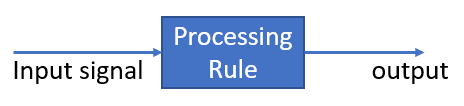
\includegraphics[width=0.5\linewidth]{Graphiken/ProcessingRule}
	\caption{General problem formulation in machine learning}
	\label{fig:ProcessingRule}
\end{figure}
There is one main difference between conventional machine learning and deep learning. While they have in common, that they get input data which is preprocessed depending on the application, in conventional machine learning features are extracted based on a defined rule \cite{Goodfellow-et-al-2016}. For this task, no theory exists and experience is necessary to choose good and relevant features for the following task, i.e. classification. The classification is done by a classifier, like kNN (k-nearest neighbour) or SVM (Support Vector Machine). In deep learning, there exists just one so-called deep neural network (DNN) for the tasks feature extraction and classification. The DNN learns and adapts the network parameters by a proper loss function. This can be obtained efficiently using the technique of (error) backpropagation (\cite{Goodfellow-et-al-2016}, \cite{Nielsen-Michael}, \cite{DeepLearningDive}, \cite{Bishop}). More details will be given in the following.\\
The learning strategy for DNNs is adapted from the way humans learn to recognize, speak, walk, calculate etc.. Despite deep learning is often seen as a exciting new technology, it can be dated back to the 1940s. Following \cite{Goodfellow-et-al-2016}, there have been three waves of development: In the 1940s-1960s (known as cybernetics), between 1980 and 1990 as connectionism and the current resurgence under the recent name deep learning beginning in 2006. The third wave of development, which is still in progress began with a breakthrough by Geoffrey Hinton. He showed that a special kind of neural network, the so called "Deep Belief Network" could be trained efficiently using a strategy called greedy layer-wise pretraining \cite{Hinton-et-al-2006}.\\
Since this breakthrough, the applications of deep neural networks increases tremendously. Examples for applications of deep neural networks nowadays are recommender systems, automatic speech recognition, text to speech translation, image recognition and/or segmentation and a lot more \cite{DeepLearningDive}. For a special task the networks are typically adjusted and the architecture is adapted. Therefore a lot of variation of deep neural networks exists nowadays, examples mentioned in \cite{Nielsen-Michael} are convolutional neural networks (CNNs), recurrent neural networks (RNNs), deep belief nets (DBNs).\\
In the following, the architecture of a feedforward neural network is exemplary showed, since "deep feedforward networks, also called feedforward neural networks or multilayer perceptrons (MLPs), are the quintessential deep learning models" \cite{Goodfellow-et-al-2016}. The naming "feedforward" comes from behaviour, that information flows in forward direction through the network, so from the input signal to the output. There is no feedback connection inside the model. These feedforward neural networks consists of multiple layers stacked together to a network. Each layer consists of many neurons. Figure \ref{fig:SingleNeuron} shows one single neuron.
\begin{figure}[htb!]
	\centering
	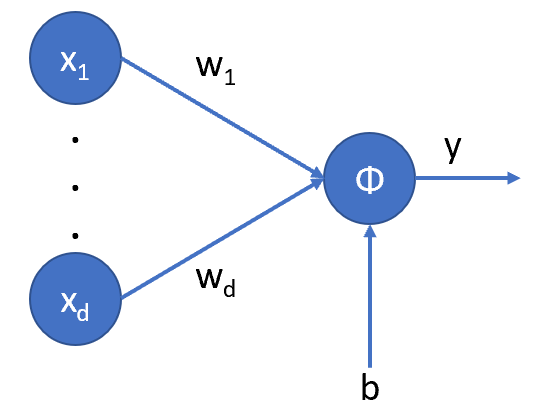
\includegraphics[width=0.3\linewidth]{Graphiken/SingleNeuron}
	\caption{Single Neuron in a feedforward neural network}
	\label{fig:SingleNeuron}
\end{figure}
In equation \ref{eq:singleneuron}, the output $y$ of a single neuron is given, with $\phi$ is the (typically non-linear) activation function of the activation $a$ which is an affine function in $\underline{x}$. $\underline{x}$ is the input vector, or the 2-d input image or 3-d input tensor. The trainable parameters of the neuron are the weights $\underline{w}$ and the bias $b$.
\begin{align}
	a = \underline{w}{^T}\underline{x}+b\\
	y = \phi(a) \label{eq:singleneuron}
\end{align}
A layer of neurons, as drawn in figure \ref{fig:Layer_of_neurons}, consists of $c$ neurons, which are connected with the input and output. The neurons in the same are not interconnected between each other. Depending on the network structure, the connections to the input and output varies. Two of the most popular layer structure are dense (or fully connected) and convolutional layer. For a dense (or fully connected) layer, each input $x_{j}$ is connected to each neuron $i$. The drawbacks of fully connected networks (FCN - network consisting of just fully connected layers) are the huge number of parameters, so a tremendous computational and memory complexity is the result. It does not learn local patterns/features of input signals since all neurons are fully connected. This problems can be solved by using a convolutional neural network (CNN - network consisting mainly of convolutional layers). Due to the properties of sparse connections and parameter sharing, the memory complexity is reduced and the networks is able to recognize input pattern regardless of its position (a CNN focusses on local input patterns) \cite{LectureNotes_DeepLearning}.
\begin{figure}[htb!]
	\centering
	\subfloat[Layer of Neurons\label{fig:NeuronsLayer}]{%			
		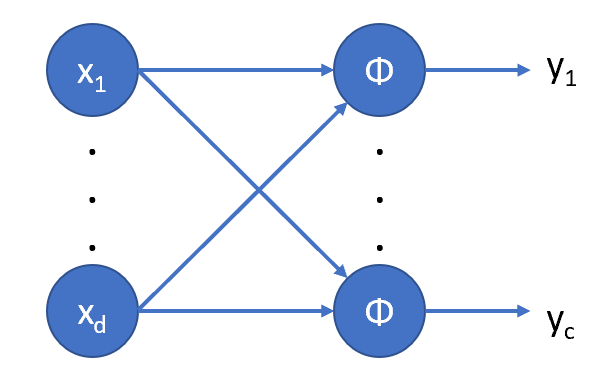
\includegraphics[width=0.45\linewidth]{Graphiken/NeuronsLayer}}
	\qquad
	\subfloat[Layer of Neurons compressed visualization\label{fig:NeuronsLayer_Matrix}]{%			
		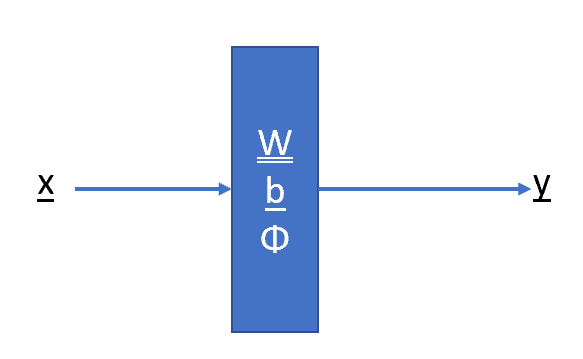
\includegraphics[width=0.45\linewidth]{Graphiken/NeuronsLayer_Matrix}}
	\caption{Layer of Neurons in feedforward neural network}
	\label{fig:Layer_of_neurons}
\end{figure}
After defining one layer, a layer can be followed by another and so on. The overall length of the chain gives the depth of the model. From this terminology, the name deep learning arose. The first layer of a network is the "input layer", while the last one is the "output layer". Those two layers have fixed sizes, since the input and the output data of a network has a defined size. All layers between them are called hidden layers. These layers are called hidden since they are neither visible to the inputs nor the outputs. Different to the the input and output layers, their size is not fixed. They are generally used to form a \textit{bottleneck}, forcing the network to make a simple model of the system with the ability to generalise to previously unseen patterns (test data) \cite{Michie-et-al-1994}. By using non-linear activation functions, such as softmax (equation \ref{eq:softmax}) or rectifier linear unit (ReLU) (equation \ref{eq:ReLU}), it can be shown that already a "two-layer MLP can approximate an arbitrary continous mapping arbitrarily closely if there is no limit to the number of hidden nodes" \cite{Michie-et-al-1994}. This property of neural networks is also known as universal function approximation.
\begin{align}
	\phi_{i}(\underline{a}) = \frac{e^{a_{i}}}{\sum_{j=1}^{c}e^{a_{j}}} \label{eq:softmax}\\
	\phi_{i}(a_{i}) = \begin{cases} a_i & a_{i} > 0\\0 & a_{i} \leq 0\\ \end{cases} \label{eq:ReLU}
\end{align}
If linear activation functions would be used, the overall network, independent on the depth of the network, will overall be just a linear transformation of the input data, so only linear solvable problems could be solved. This shows the importance for choosing non-linear activation functions.\\
For training a neural network, a loss function based on the training data has to be defined, which has to be minimized, with respect to the network parameters. 
Overall, the training task for a neural network is to minimize the cost function $L(\underline{\theta})$ on the training data as given in equation \ref{eq:CostFunction} with $\iota(\underline{x}(n),\underline{y}(n);\underline{\theta})$ is an arbitrary loss function where $\underline{y}$ is the target output of the network and $\underline{x}$ is the input of the network. The cost function denotes the total loss over all $N$ samples.
\begin{align}
	\underset{\underline{\theta}}\min L(\underline{\theta}) = \frac{1}{N}\sum_{n=1}^{N}\iota(\underline{x}(n),\underline{y}(n);\underline{\theta})  \label{eq:CostFunction}
\end{align}
The loss function is depending on the task. For regression, a typical loss function is the $l_{2}$-loss, where $l_{2}$-Norm of the error is used. The error is the difference between the target output $\underline{y}$ and the output of the neural network, $f(\underline{x};\underline{\theta})$. This loss function is given in equation \ref{eq:l2-loss}.
\begin{align}
	\iota(\underline{x},\underline{y};\underline{\theta}) = ||\underline{y}-f(\underline{x};\underline{\theta})||^{2}\label{eq:l2-loss}
\end{align}
For classification, a typical loss function is the categorical loss. Equation \ref{eq:cat-loss} denotes this loss function.
\begin{align}
	\iota(\underline{x},\underline{y};\underline{\theta}) = -\underline{y}^{T}ln f(\underline{x};\underline{\theta})\label{eq:cat-loss}
\end{align}
Our target is to find $\underset{\underline{\theta}}\min L(\underline{\theta})$, which has in general no closed-form solution. Therefore, numerical minimization is used in deep learning. The standard algorithm for minimizing the loss function is the gradient descent (GD) algorithm. In this algorithm, the gradient information is used to choose the parameter update to comprise a small step in the direction of the negative gradient \cite{Bishop}. Equation formulates the update step of the GD-algorithm where $t \in \mathbb{Z}_{\geq0}$ is the iteration index and $\eta > 0$ is the step size or learning rate. $\underline{\theta}^{0}$ is the initialization of the network and an initial guess for $\theta$.
\begin{align}
	\underline{\theta}^{t+1} = \underline{\theta}^{t} - \eta\underline{\nabla}L(\underline{\theta})|_{\underline{\theta}=\underline{\theta}^{t}}\label{eq:GradientDescent_update}
\end{align}
Due to the size training datasets, not the whole dataset can be kept in the memory. Therefore stochastic gradient descent is used to reduce the computing cost for each iteration, where the gradient vector $\underline{\nabla}L$ and the update $\underline{\theta}$ is calculated for one minibatch $i$. The stochastic gradient $\underline{\nabla}L_{i}$ is the unbiased estimate of the gradient $\underline{\nabla}L$, so we have a more noisy gradient which lead to the name \textbf{stochastic} gradient descent \cite{DeepLearningDive}.\\
It is obvious, that the calculation of $\underline{\nabla}L$ is crucial for performing an update step. Therefore, we want to compute the partial derivatives of the cost function with respect to the network parameters $w$ and $b$: $\dfrac{\partial L}{\partial w}$ and $\dfrac{\partial L}{\partial b}$. This can be done efficiently by using the error backpropagation algorithm (sometimes just called \textit{backpropagation} or \textit{backprop}). As the name denotes, the error vector are backpropagated through the network. Starting at the output layer, the  error vector of layer $L$ with respect to the weights $w_{L_{ij}}$ is given in equation \ref{eq:ErrorVector_OutputLayer} with $\underline{x}_{L}$ as the output and $\underline{a}_{L}$ as activation of layer $L$. Calculating the partial derivative with respect to $b$ follows the same algorithms.
\begin{align}
	\underline{\delta}_{L}^{T} = \dfrac{\partial L(\underline{\theta})}{\partial w_{L_{ij}}} = \dfrac{\partial L}{\partial \underline{x}_{L}}\dfrac{\partial \underline{x}_{L}}{\partial \underline{a}_{L}}\dfrac{\partial \underline{a}_{L}}{\partial w_{L_{ij}}}\label{eq:ErrorVector_OutputLayer}
\end{align}
For the remaining layers $l \in [1, L-1]$ the error vector can be calculated by applying the chain rule for differentiation. The error vector for layer $l$ can be calculated with equation \ref{eq:ErrorVector_generalLayer} \cite{LectureNotes_DeepLearning}.
\begin{align}
	\underline{\delta}_{l}^{T} = \underline{\delta}_{l+1}^{T}\dfrac{\partial \underline{a}_{l+1}}{\partial a_{l}}\dfrac{\partial \underline{a}_{l}}{\partial w_{l_{ij}}}\label{eq:ErrorVector_generalLayer}
\end{align}
Figure \ref{fig:Backprop_DNN} gives a graphical representation of the paths through a DNN. Figure \ref{fig:ForwardPass_DNN} shows the forward path through a DNN for calculating the cost values. Figure \ref{fig:BackwardPass_DNN} shows the backpropagation of the error vectors through the network.
\begin{figure}[htb!]
	\centering
	\subfloat[Layer of Neurons\label{fig:ForwardPass_DNN}]{%			
		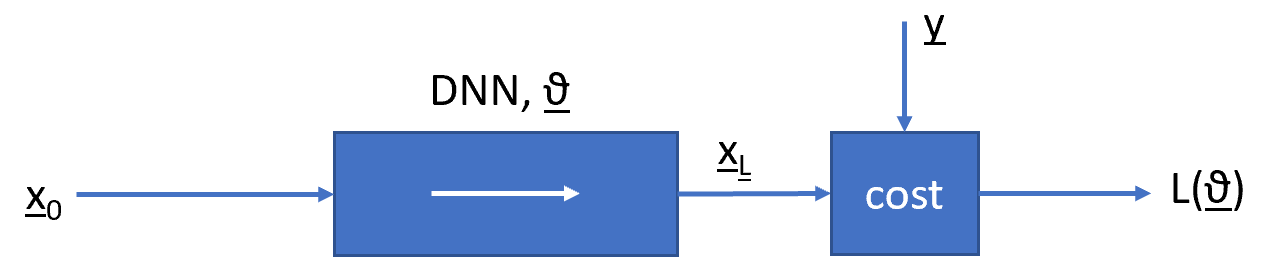
\includegraphics[width=0.45\linewidth]{Graphiken/ForwardPass_DNN}}
	\qquad
	\subfloat[Layer of Neurons compressed visualization\label{fig:BackwardPass_DNN}]{%			
		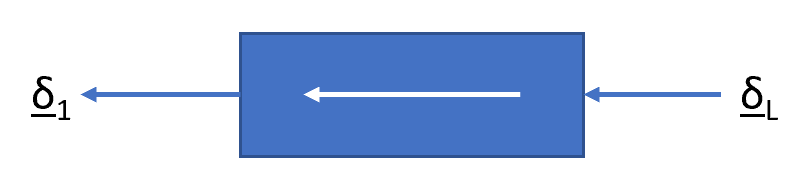
\includegraphics[width=0.45\linewidth]{Graphiken/BackwardPass_DNN}}
	\caption{Layer of Neurons in feedforward neural network}
	\label{fig:Backprop_DNN}
\end{figure}
By backpropagating through the network, $\underline{\delta}_{1}^{T}$ gives in the end the error vector of the network. This information will then be used for updating the weights and biases following an numerical optimization algorithm like the stochastic gradient descent algorithm.\\
\cite{Bishop} summarizes the error backpropagation in four steps:
\begin{enumerate}
	\item Apply the input $\underline{x}_{0}$ to the network and forward propagate through the network as in figure \ref{fig:ForwardPass_DNN} to find activations of all the hidden and output units.
	\item Evaluate the error vector $\underline{\delta}_{L}^{T}$ for all output units using equation \ref{eq:ErrorVector_OutputLayer}
	\item Backpropagate the error vectors through $\underline{\delta}_{l}^{T}$ the network following \ref{eq:ErrorVector_generalLayer} to obtain the error vector for each hidden unit in the network (figure \ref{fig:BackwardPass_DNN})
	\item Apply a numerical optimization algorithm (i.e. SGD) to adapt the network parameters
\end{enumerate}
Training (optimizing) a neural network is a difficult task and suffers from a number of optimization difficulties. Table \ref{tab:Difficulties} gives a rough summary about the difficulties and solutions in optimizing a neural network \cite{LectureNotes_DeepLearning}.\\
\begin{table}
    \centering
    \caption{Difficulties in optimizing a neural network}
    \label{tab:Difficulties}
    \begin{tabular}{lcc}
        \toprule
        Difficulty & Solutions\\
        \midrule
        stochastic gradient & larger minibatch size, momentum\\
        ill conditioning & momentum, input scaling and batch normalization\\
        saddle point / plateau & noisy gradient\\
        sensitive to step size & learning rate schedule\\
        local minimum & parameter initialization\\
        vanishing gradient & parameter initialization, improved model\\
        \bottomrule
    \end{tabular}
\end{table}
As mentioned in \cite{DeepLearningDive}, optimization provides a way to minimize the loss function for deep learning, but, in essence, the goals of optimization and deep learning are different. In pure optimization, we want to minimize the (training) loss function. But in deep learning, we focus on minimizing the generalization error, which is the value of the loss function computed on new, unseen data (test data). Thus it is important to regularly apply test data to the network while training, to see if the network is overfitted to the training data. This means, the error on the training data is very small in comparison to the test/generalization error. There are various methods to ensure overfitting does not take place, i.e. dropout or regularization (\cite{Goodfellow-et-al-2016}, \cite{Nielsen-Michael}, \cite{DeepLearningDive}, \cite{Bishop}).\\
\section{Unsupervised Learning}
This chapter will give an overview of unsupervised learning and will go into more detail about two main tasks of unsupervised learning: dimensionality reduction/representation learning and clustering.\\
Unsupervised learning offers the possibility of exploring structure of data without guidance in the form of class information, which leads to the name "unsupervised". In comparison to supervised or semi-supervised learning, no class information (no labels) are available while training. This can "often reveal features not previously expected or known about" \cite{Michie-et-al-1994}.\\
In the task dimensionality reduction or representation learning, the task is to find a representation of the original data in a lower dimensional feature space. So it offers a model of the data in fewer parameters than were required to store the entire training dataset. This has big advantages for storing, coding and transmitting data. After learning the hidden representations by an encoding and decoding form, some models are able to generate new data with same characteristic as the original data when required. These models are called generative models.\\
When having datasets without labels, in most applications it is relevant to cluster similar data points together. Therefore clustering can be applied. Intuitively, it is assumed that inter-points similarities are high in a group of data points which belong to the same cluster and vice-versa. The similarity measure could be any kind of measure, i.e. euclidean distance or a probability value (probability belonging to a cluster). Popular clustering techniques are K-means clustering \cite{Lloyd82leastsquares}, DBSCAN \cite{Ester96adensity-based} or Gaussian Mixture Model (GMM) \cite{Gilles07MixtureModelsforClassification}. In Image segmentation, the original image has already a high dimensional. Even "small" pictures, i.e. 32x32 images, have a 1024-dimensional feature space. In a high-dimensional feature space, similarity measures as euclidean distance are getting weaker to find similarities, also known as the course of dimensionality (first introduced by \cite{Bellman34}). Due to this, and the idea of clustering data based on relevant extracted features, the state-of-the art for clustering is not using the original data, but extract relevant features by applying dimensionality reduction/representation learning to the data, and use a clustering algorithm on the "bottleneck" representation of the data (the so called latent space).
\subsection{Dimensionality Reduction/Representation Learning}
As mentioned above, we want to reduce the dimensionality of the original data but still have meaningful representations of it. Generally, we want a good representation of the data, which is "one that makes a subsequent learning task easier" \cite{Goodfellow-et-al-2016}. In the objective of this work, the subsequent learning task is classification. In this work, we use autoencoder models and variations of it for this task. Figure \ref{fig:Autoencoder} illustrates the general architecture of an autoencoder with input image $\underline{x}$, the latent representation $\underline{z}$ of the data and the reconstructed image $\underline{\hat{y}}$. As ground truth for the loss calculation the original image is used and compared to the reconstructed one. This loss is called the reconstruction loss $L_{r}$.
\begin{figure}[htb!]
	\centering
	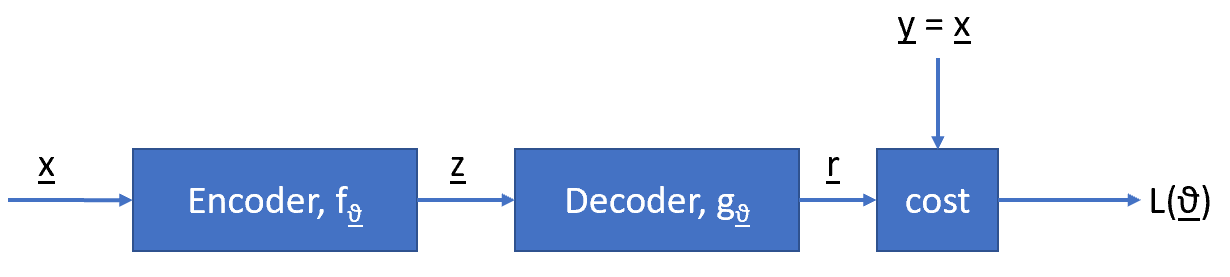
\includegraphics[width=0.6\linewidth]{Graphiken/Autoencoder_Architecture}
	\caption{General architecture of an autoencoder}
	\label{fig:Autoencoder}
\end{figure}
As seen in figure \ref{fig:Autoencoder}, the autoencoder consists of two parts, the encoder and decoder. The encoder can be seen as feature-extracting function $f_{\underline{\theta}}$ which will allow a straightforward and efficient computation of a feature vector $\underline{z} = f_{\underline{\theta}}(\underline{x})$ from an input $\underline{x}$. For each sample $\underline{x}(n), n \in [1,N]$ we define $\underline{z}(n)$ as our feature-vector/representation/code/embedding or latent variable from $\underline{x}(n)$ (see equation \ref{eq:Embedding_z}). 
\begin{align}
	\underline{z}(n) = f_{\underline{\theta}}(\underline{x}(n))\label{eq:Embedding_z}
\end{align}
The decoder function $g_{\underline{\theta}}$ maps from latent space back into the original input space producing the so-called reconstruction $\underline{r}$, which is defined in equation \ref{eq:Reconstruction}.
\begin{align}
	\underline{r} = g_{\underline{\theta}}(\underline{z}) = g_{\underline{\theta}}(f_{\underline{\theta}}(\underline{x}(n)))\label{eq:Reconstruction}
\end{align}
The set of parameters $\underline{\theta}$ of the encoder and decoder are learned simultaneously on the task of reconstructing the original input as well as possible, minimizing the reconstruction loss $L_{r}(\underline{x},\underline{r})$.\\
Mostly (also in this work), undercomplete or regularized autoencoders are used. These architectures ensure a dimensionality reduction by using a bottleneck, i.e. $d_{\underline{z}} << d_{\underline{x}}$. This one the one hand clearly achieves a dimensionality reduction, but this architecture is also helpful in terms of overfitting. When $d_{\underline{z}} \geq d_{\underline{x}}$, this can allow the autoencoder to simply duplicate the input in the features, thus achieving (nearly) perfect reconstruction without having extracted more meaningful features \cite{Bengio-et-al-2013}.\\
In our work, we focus on achieving meaningful latent representations $\underline{z}$ since these latent representations will further be used as input for our clustering step. More details about the detailed architecture of the dimensionality reduction/representation learning part of our model will be discussed in the corresponding sections.
\subsection{Clustering algorithm}
The main objective of clustering is to separate data into groups of similar data points. Clustering algorithms have in principal be able to answer two questions:
\begin{enumerate}
	\item Which samples belongs to the same cluster?
	\item How man clusters exist in the dataset?
\end{enumerate}
Based on these questions, we can split between two kinds of clustering algorithms. The first kind of algorithm can't answer question 2. They need as a-priori information the number of clusters in the dataset. Examples for this kind of algorithms are k-means \cite{Lloyd82leastsquares}, fuzzy c-means \cite{Bezdek81fuzzycmenas} or Gaussian Mixture Model (GMM) \cite{Gilles07MixtureModelsforClassification}.\\
The second kind does not need this information, these algorithms are constructed to find the number of clusters while the clustering process by itself. Examples for this kind of algorithms are DBSCAN \cite{Ester96adensity-based} or mean-shift clustering \cite{Fukunaga75mean-shift}.\\
In this work, the clustering algorithms k-means and GMM are used, since they are typically used for the clustering step in state-of-the-art clustering models. These two algorithms will be explained in more detail in the following sub sections.
\subsubsection{K-means Clustering}
As already described the problem for clustering is identifying groups (or clusters) of data points in a d-dimensional space. Given the number of clusters as $K$, big inter-samples similarities within a cluster compared to the samples of another cluster are desired. To measure the similarity from a sample to a cluster a cluster representation, the cluster center $\underline{\mu}_{k}$ for each cluster, is defined. Following this, the samples are assigned to the clusters, which will be done by assigning each sample to the cluster with the nearest center (nearest-mean assignment). This will be expressed by a binary indicator variable $r_{nk}$, where $r_{nk} = 1$ if the sample $\underline{x}_{n}$ is assigned to cluster $k$ and $r_{nk} = 0$ otherwise. After this, an objective function can be defined, given in equation \ref{eq:kMeans_Objective} with $sim(\underline{x}_{n}, \underline{\mu}_{k})$ could be any similarity or dissimilarity metric (i.e. euclidean distance or cosine similarity).
\begin{align}
J = \sum_{n=1}^{N} \sum_{k=1}^{K} r_{nk} sim(\underline{x}_{n}, \underline{\mu}_{k})\label{eq:kMeans_Objective}
\end{align}
As an example, the squared euclidean distance is chosen as dissimilarity metric (equation \ref{eq:squared_euclidean_distance}).
\begin{align}
sim(\underline{x}_{n}, \underline{\mu}_{k}) = ||\underline{x}_{n} - \underline{\mu}_{k}||^{2}\label{eq:squared_euclidean_distance}
\end{align}
Having a measure for the dissimilarity, we can define the cluster assignment as following (equation):
\begin{align}
r_{nk} = \begin{cases} 1 & if\ k = arg\ \underset{j}\min ||\underline{x}_{n} - \underline{\mu}_{j}||^{2}\\0 & otherwise\end{cases}\label{eq:sample_clusterassignment}
\end{align}
Using the defined formulas, the goal is to find values for $r_{nk}$ and $\underline{\mu}_{k}$ to minimize $J$. This can be done by an iterative procedure where every iteration contains of two steps. First fix $\underline{\mu}_{k}$ and assign the samples to the cluster centers, so update $r_{nk}$ to minimize J. In the second step fix $r_{nk}$ and update $\underline{\mu}_{k}$. This can be done for a defined number of iterations or until convergence (no change in cluster assignments) \cite{Bishop}.\\
The algorithm is summarized in the following \cite{LectureNotes_DPR}:
\begin{description}
	\item[Given]\hfill \\
		samples $S = \lbrace\underline{x}_{1},...,\underline{x}_{N}\rbrace$
	\item[Parameter]\hfill \\
		number of clusters $k$
	\item[Initialization]\hfill \\
		Initialization of cluster centers\\
		$i = 0$
	\item[Do]\hfill
		\begin{itemize}
			\item get $k$ clusters $S_{i}$ by assigning each $\underline{x}_{n}$ to the nearest center (mean of cluster) $\underline{\mu}_{j}$ (nearest-mean classifier)
			\item recompute the cluster centers (equation \ref{eq:cluster_center_update})
				\begin{align}
					\underline{\mu}_{j} = \dfrac{1}{|S_{i}|} \sum_{\underline{x}_{n} \in S_{i}}\underline{x}_{n}\label{eq:cluster_center_update}
				\end{align}
			\item i+1
		\end{itemize}
	\item[Until] no change in clusters $S_{i}$ or $i \geq max\_iter$
\end{description}
It is obvious, that the convergence time of the algorithm is sensitive to the choice of the initial cluster centers. An naive (and fast) approach is to randomly choose samples out of $S$ to initialize the cluster centers. Nevertheless, there are more improved initialization schemes available (\cite{Yi10ImprovedInitialization}, \cite{Arthuer07kmeans_plusplus}).
\subsubsection{Gaussian Mixture Model}
Gaussian Mixture Models (GMMs) can be used for clustering. It is a probabilistic approach. Each cluster will be described by its estimated centroids (or mean) $\hat{\underline{\mu}}_m$, estimated covariance matrix $\hat{\mathbf{C}}_m$ and the mixture weights $\hat{\alpha}_m$ with $\sum_{m=1}^{M}\hat{\alpha}_m=1$, which can be interpreted as estimated (relative) size of the clusters. Instead of identifying cluster assignments by determine the "nearest" (or most similar) cluster (as in k-means), we fit a set of $M$ Gaussian distributions to the data. The number of applied gaussians $M$ is also called the model order. The above introduced parameters of the distributions are learned by the EM-algorithm \cite{Dempster-et-al-1977}. After learning this parameters, we can calculate the probabilities of each sample and perform an assignment based on these probability values. The probability density function $p_m$ follows a normal distribution as in equation \ref{eq:GMM_distribution} \cite{Bishop}.
\begin{align}
	p_m(\underline{x}_n) = \hat{\alpha}_m\mathcal{N}(\underline{x}_n|\hat{\underline{\mu}}_m, \hat{\mathbf{C}}_m)\label{eq:GMM_distribution}
\end{align}
The probability of a sample $\underline{x}_n$ belonging to the cluster $m$ is the corresponding posterior probability $q_{m,n} = P(z_n = m|\underline{x}_n;\hat{\underline{\theta}})$ with $z_n$ is the assignment of sample $\underline{x}_n$ to cluster $m$. So this denotes the probability for sample $\underline{x}_n$ belonging to cluster $m$. The posterior can now be calculated with formula \ref{eq:GMM_distribution}, leading to equation \ref{eq:GMM_posterior}.
\begin{align}
	q_{m,n} = \dfrac{\hat{\alpha}_mp_m(\underline{x}_n|\hat{\underline{\theta}}_m)}{\sum_{m=1}^{M}\hat{\alpha}_mp_m(\underline{x}_n|\hat{\underline{\theta}}_m)}\label{eq:GMM_posterior}
\end{align}
The estimated mixture weights $\hat{\alpha}_m$ can be thus calculated as in equation \ref{eq:GMM_mixtureweights} with formula \ref{eq:GMM_posterior}.
\begin{align}
	\hat{\alpha}_m = \dfrac{1}{N}\sum_{n=1}^{N}q_{m,n}\label{eq:GMM_mixtureweights}
\end{align}
Another weight parameter, $w_{m,n}$ is introduced. This weight parameter is defined for each sample/cluster combination. It can be seen as a posterior probability, that the component $m$ was responsible for generating $\underline{x}_n$ \cite{Bishop}. Formula \ref{eq:GMM_sampleweights} shows the calculation of $w_{m,n}$.
\begin{align}
	w_{m,n} = \dfrac{q_{m,n}}{\sum_{n=1}^{N}q_{m,n}}\label{eq:GMM_sampleweights}
\end{align}
After defining the weight parameter $w_{m,n}$ we can now update the corresponding parameters from the defined Normal distribution. Therefore, the mean vector (equation \ref{eq:GMM_meanupdate}) and the covariance matrix (equation \ref{eq:GMM_covarianceupdate}) are updated for each cluster $m$.
\begin{align}
	\hat{\underline{\mu}}_m = \sum_{n=1}^{N}w_{m,n}\underline{x}_n\label{eq:GMM_meanupdate}\\
	\hat{\mathbf{C}}_m = \sum_{n=1}^{N}w_{m,n}(\underline{x}_n-\hat{\underline{\mu}}_m)(\underline{x}_n-\hat{\underline{\mu}}_m)^{T}\label{eq:GMM_covarianceupdate}	
\end{align}
The above introduced formulas can now be executed iteratively, which then leads to the Expectation Maximization algorithm, also denoted as EM-algorithm. It can be done until a given number of iterations is reached or the update step $||\hat{\underline{\theta}}(k+1) - \hat{\underline{\theta}}(k)||$ is below a certain threshold. In the following the EM-algorithm is shortly summarized \cite{LectureNotes_DPR}.
\begin{description}
	\item[Given]\hfill \\
		N samples $\underline{x}_{1},...,\underline{x}_{N}$
	\item[Parameter]\hfill \\
		model order (number of clusters) $M$
	\item[Initialization]\hfill \\
		$\hat{\alpha}_m(0),\ \hat{\underline{\mu}}_m(0),\ \hat{\mathbf{C}}_m(0)$ ($1 \leq m \leq M)$\\
		$k = 0$
	\item[Do]  for $1 \leq m \leq M$ and $1 \leq n \leq N$\hfill
		\begin{itemize}
			\item calculate the posterior $q_{m,n}(k)$ by equation \ref{eq:GMM_posterior} with $\hat{\alpha}_m(k)$ and $\hat{\underline{\theta}}_m(k)$
			\item calculate $\hat{\alpha}_m(k+1)$ by equation \ref{eq:GMM_mixtureweights} with $q_{m,n}(k)$
			\item calculate $w_{m,n}(k)$ by equation\ref{eq:GMM_sampleweights} with $q_{m,n}(k)$
			\item calculate $\hat{\underline{\mu}}_m(k+1)$ by equation \ref{eq:GMM_meanupdate} with $w_{m,n}(k)$
			\item calculate $\hat{\mathbf{C}}_m(k+1)$ by equation \ref{eq:GMM_covarianceupdate} with $w_{m,n}(k)$ and $\hat{\underline{\mu}}_m(k+1)$
			\item k+1
		\end{itemize}
	\item[Until] $||\hat{\underline{\theta}}(k+1) - \hat{\underline{\theta}}(k)|| < threshold$ or $i \geq max\_iter$
\end{description}
It should be mentioned that there is no guarantee that the EM algorithm will converge to the desired global maximum of the likelihood, but it is ensured, that each iteration of the EM algorithm will not decrease the value of the likelihood.\\
After the EM algorithm, the samples $\underline{x}_n$ can be clustered by using the GMM parameters. Each samples will be assigned to the cluster for which the sample has its highest posterior probability $q_{m,n}$, as given in formula \ref{eq:GMM_Clusterassignment}, which corresponds to a Maximum-Likelihood decision.
\begin{align}
	arg\ \underset{m}\max\ q_{m,n}\label{eq:GMM_Clusterassignment}
\end{align}
The convergence of the EM algorithm directly depends on its initialization. In general, an improvement can be achieved by repeating the initialization several time and select the best GMM parameter estimate. A possible way to find the initial values $\hat{\alpha}_m(0),\ \hat{\underline{\mu}}_m(0),\ \hat{\mathbf{C}}_m(0)$ ($1 \leq m \leq M)$ is choosing randomly $M$ samples from all $N$ training samples as initial guess for $\hat{\underline{\mu}}_m(0)$. $\hat{\mathbf{C}}_m(0)$ are assumed to be diagonal and identical. The diagonal elements of $\hat{\mathbf{C}}_m(0)$ are then estimated from the sample variances of the $M$ selected training samples. For the initial mixture weights, a uniform distribution of the clusters is assumed, so $\hat{\alpha}_m(0) = 1/M$. Another possibility for initialization is using k-means clustering first to find initial values for the initial means $\hat{\underline{\mu}}_m(0)$ and then continue as above \cite{LectureNotes_DPR}.
\chapter{Working Environment (Framework)}
In this chapter the working environment for evaluating the models is introduced. First, the software environment, namely TensorFlow, is introduced in a section. Secondly, the framework, which was developed in beginning of this work, is introduced and the general architecture.
\paragraph{TensorFlow}\mbox{}\\
TensorFlow is an interface for expressing machine learning algorithms, and an implementation for executing such algorithms. It is a system that was developed to operate at large scale and in heterogeneous environments. The focus of TensorFlow is on training and inference on deep neural networks. It uses dataflow graphs to represent computation, shared state and the operations \cite{tensorflow2015-whitepaper}. In this work, the TensorFlow Version 1.13 is used.
\paragraph{Framework}\mbox{}\\
The implemented framework is used to have an easy comparison of different models, i.e. in using the same training procedure and same evaluation metrics. Therefore, the implementation has to be as modular as possible, so that new architectures could easily be implemented and evaluated. But on the other side, clear interfaces are defined for every model so that a general training algorithm can be used which allows comparability. The program flow is as following:
\begin{enumerate}
	\item Parameters are set in a separate parameter file
	\item The inputs for the models are defined. Separate inputs are created for the training and clustering part. An iterator with the desired attributes (i.e. batch-size, shuffling, resizing, data augmentation) is returned 
	\item The \textit{train model} is created, which is the model to extract features out of the original data. The \textit{train model spec} is returned containing the necessary operations (i.e. initialization, optimization, metric updates etc.) and the interface to the latent representation for clustering
	\item The \textit{cluster model} is created, which is the model to cluster the data based on the latent representation of the \textit{train model}. The \textit{cluster model spec} is returned containing the necessary operations (i.e. initialization, cluster adjustments, cluster assignments, metric updates etc.).
	\item The created models are transmitted to a function for training and evaluation. This training and evaluation step is repeated until the defined number of epochs is reached.
		\begin{description}
			\item[Training:] Execute the training operation of the \textit{train model} for one iteration over the whole training data, update the defined metrics and write them to the Tensorboard
			\item[Evaluation:] The clustering is executed on all clustering data and the corresponding metrics are calculated and written to Tensorboard. If selected, the latent space is visualized in a 2-dimensional space with the help of UMAP \cite{mcinnes2018umap-software} and t-SNE \cite{t-SNE}.			
		\end{description}
\end{enumerate}
The desired dataset, feature extraction model and clustering algorithm is selected when executing the program by argument parsers. Based on the selected combination and time, the summaries from training and evaluation are stored in a folder with unique naming. Also the parameters are stored there, so the results can be reproduced easily. The implemented models will be introduced in the next chapter.
\chapter{Preliminary Architectures and Algorithm}
\section{Autoencoder}
\section{Variational Autoencoder}
\section{IDEC}
\chapter{Experimental Setup}
\section{Datasets}
\section{Investigated Hyperparameters}
\chapter{Results}
\chapter{Summary and Outlook}

\appendix
\chapter{Additionally}
You may do an appendix

	% -------------------> end writing here <------------------------
	% *****************************************************************
	\ifthenelse{\equal{\doclang}{german}}{
		\bibliographystyle{IEEEtran_ISSger}
	}{
		\bibliographystyle{IEEEtran_ISS}
	}
	\bibliography{refs}
	
	% *****************************************************************
	%% Additional page with Declaration ("Eidesstattliche Erklrung");
	%% completed automatically
	\begin{titlepage}
		\vfill
		\LARGE \ifthenelse{\equal{\doclang}{german}}{\textbf{Erkl\"arung}}{\textbf{Declaration}}
		\vfill
		
		\ifthenelse{\equal{\doclang}{german}}{
			Hiermit erkl\"are ich, dass ich diese Arbeit selbstst\"andig verfasst und keine anderen als die angegebenen
			Quellen und Hilfsmittel benutzt habe.
		}
		{
			Herewith, we declare that we have developed and written the enclosed thesis entirely by ourself and that I have not used sources or means except those declared.
		}
		
		\vspace{1cm}
		
		\ifthenelse{\equal{\doclang}{german}}{
			Die Arbeit wurde bisher keiner anderen Pr\"ufungsbeh\"orde vorgelegt und auch noch nicht ver\"offentlicht.
		}
		{
			This thesis has not been submitted to any other authority to achieve an academic grading and has not been published elsewhere.
		}
		
		\vfill
		
		
		Stuttgart, \signagedate
		\hfill
		\begin{tabular}{l}
			\hline
			\student
		\end{tabular}
	\end{titlepage}
	
	
	
\end{document}
